% ----------------------------------------------------------
% Teste test3_3_e25b32class10_20231211_234419
% ----------------------------------------------------------
\subsubsection{Teste test3_3_e25b32class10_20231211_234419 - AlexNet (Is That a Santa)}

Informações utilizadas para o treinamento.

\begin{table}[ht]
   \centering
   \caption{Treinamento}
   \label{tab:modelos}
   \begin{tabular}{| c | c | }
      \hline 
      \textbf{Informação} & \textbf{Descrição} \\
      \hline \hline 
      Rede & AlexNet \\
      \hline
      Número de épocas & 25\\
      \hline
      Tamanho do lote & 32\\
      \hline
      Taxa inicial & 0.012 \\
      \hline
      Taxa de decaimento & 0.0006 \\
      \hline
      Total de classes & 10\\
      \hline
      Dataset & CIFAR-10\\
      \hline
   \end{tabular} 
\end{table}

Resultados obtidos após treinamento.

\begin{tabular}{lrrrr}
\toprule
  Unnamed: 0 &  precision &  recall &  f1-score &  support \\
\midrule
    airplane &   0.871508 &   0.780 &  0.823219 &  1000.00 \\
  automobile &   0.936126 &   0.894 &  0.914578 &  1000.00 \\
        bird &   0.776923 &   0.707 &  0.740314 &  1000.00 \\
         cat &   0.638298 &   0.690 &  0.663143 &  1000.00 \\
        deer &   0.822060 &   0.790 &  0.805711 &  1000.00 \\
         dog &   0.768053 &   0.702 &  0.733542 &  1000.00 \\
        frog &   0.898343 &   0.813 &  0.853543 &  1000.00 \\
       horse &   0.841651 &   0.877 &  0.858962 &  1000.00 \\
        ship &   0.751001 &   0.938 &  0.834149 &  1000.00 \\
       truck &   0.835478 &   0.909 &  0.870690 &  1000.00 \\
    accuracy &   0.810000 &   0.810 &  0.810000 &     0.81 \\
   macro avg &   0.813944 &   0.810 &  0.809785 & 10000.00 \\
weighted avg &   0.813944 &   0.810 &  0.809785 & 10000.00 \\
\bottomrule
\end{tabular}


\begin{figure}[ht]
 \begin{center}
   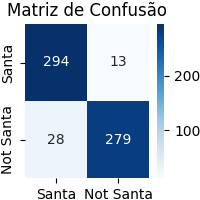
\includegraphics[scale=1]{tests/test3_3_e25b32class10_20231211_234419/confusion_matrix.png}
  \caption{Matriz de Confusão}
  \label{fig:fig03}
 \end{center}
\end{figure}

\begin{figure}[ht]
 \begin{center}
   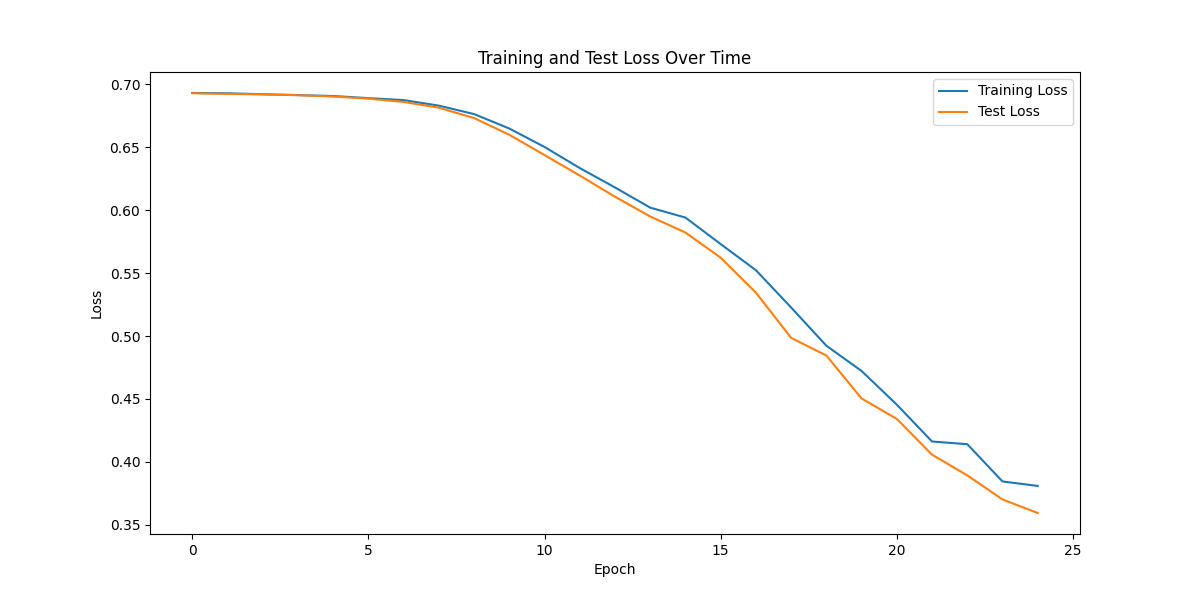
\includegraphics[scale=0.8]{tests/test3_3_e25b32class10_20231211_234419/loss_over_time.png}
  \caption{Gráfico de Perda}
  \label{fig:fig04}
 \end{center}
\end{figure}
